% !TeX root = ../main.tex
% Add the above to each chapter to make compiling the PDF easier in some editors.

\chapter{Background}\label{chapter:background}

\section{Verifiable Credentials}

\acrfull{VC} is a recent \acrshort{W3C} standard for interoperable digital credentials on the Web that is cryptographically secure, tamper-evident, privacy respecting, and machine-verifiable" \parencite{Sporny.18Kas2019}. These credentials include but are not limited to passports, ID cards, university degrees, tickets etc. Any set of claims about a subject can be a credential. In the \acrshort{VC} setting these claims create \textit{subject-property-value} relationships that can be expressed in graphs. For instance being graduated from a university can be represented as the graph in Figure \ref{fig:alumniOf}. 

Subjects of claims are not necessarily persons and can be anything. In a peer review context a claim could be \textit{Peer Review-author-John Doe} where the subject is the peer review. Alternatively same relationship can be represented as \textit{John Doe-reviewerOf-Peer Review} where the subject is the person.

\begin{figure}[htbp]
  \centering
  \includesvg[width=0.8\textwidth]{claim-example}
  \caption{Example Subject-Property-Value relationship of a graduation claim \parencite{Sporny.18Kas2019}} \label{fig:alumniOf}
\end{figure}

Although people usually associate credentials to be issued only by a respected authority such as a state, a university or a hospital, \acrlong{VC} allows anyone to issue claims. Yet, each credential is meaningful in a certain context and depending on the trust relationships between parties. An \textit{alumniOf} claim is only meaningful if issued by a university that is known to the employer in a job application or a \textit{goodHusband} claim only makes sense if issued by a spouse. Parties that receive a credential can choose to accept or reject a credential depending on the real world trust relationships.

A credential is a set of claims, i.e. a graph of information around a subject. Additional to the claims, the metadata and a digital proof form a verifiable credential. The proof is generally a digital signature of the claims and metadata, which makes the verifiable credential "verifiable".

\begin{figure}[htbp]
  \centering
  \includesvg[width=0.4\textwidth]{credential}
  \includesvg[width=0.8\textwidth]{credential-graph}
  \caption{Components of a verifiable credential and the graph of information of an example credential \parencite{Sporny.18Kas2019}} \label{fig:credentialGraph}
\end{figure}

The \acrshort{VC} specification models the stakeholders and interactions between them as in Figure \ref{fig:ecosystem}. \textit{Issuer}s assert claims and issue credentials about subjects, \textit{Verifier}s verify the credentials presented to them, and \textit{Holder}s aquire, store, and present credentials. Note that the subject of a credential can be different than its holder such as a pet being the subject and its owner being the holder, or a peer review as the subject and the reviewer as the holder. Finally, a \textit{Verifiable Data Registry} acts as the backend of these interactions by maintaining identifiers and schemas. This registry could be a distributed ledger or a central database depending on the implementation.

\begin{figure}[htbp]
  \centering
  \includesvg[width=0.8\textwidth]{ecosystem}
  \caption{Stakeholders of a \acrlong{VC} ecosystem and their roles \parencite{Sporny.18Kas2019}} \label{fig:ecosystem}
\end{figure}

\subsection{Verifiable Presentations}

The specification also describes an extension to the \acrshort{VC} data model that enables the packaging of multiple credentials and verification of the authorship of the data. A Verifiable Presentation consists of one or more verifiable credentials, presentation metadata, and a proof which is usually a digital signature of the first two. Credential holders can combine different credentials from different issuers for each use case, and the proof of the presentation provides the means to verify the authorship of data.

\subsection{Syntax}

The data model provided in the \acrshort{VC} specification is an abstract representation of the information around a credential. For the exchange of the information a machine readable data exchange format or syntax is required. Popular data exchange formats are XML \parencite{xmlRFC}, \acrshort{JSON} \parencite{jsonRFC}, and \acrshort{YAML} \parencite{yaml}. Although any syntax can be used, the specification describes \acrfull{JSON-LD} \parencite{jsonld} and \acrshort{JSON} with \acrshort{JWT} \parencite{rfc7519} serializations of the data model. \acrshort{JSON-LD} is the preferred format for many applications including this work. A comparison of \acrshort{JSON-LD} over \acrshort{JWT} is available in the \acrshort{VC} implementation guide and is discussed in \cite{young_2021}. 

\acrshort{JSON-LD} is both an extension to \acrshort{JSON} and effectively a \acrfull{RDF} \parencite{rdf} syntax. The use of \acrshort{JSON-LD} accomplishes several things. First, it  brings linked data properties with minimal changes to \acrshort{JSON}, which is widely used in today's web. Second, it makes possible to model complex real world relationships with a graph model. Third, it enables "permissionless innovation" through extensibility. Anyone can extend the existing vocabularies and numerous cryptographic proof formats and signature suites can be used. This is in line with the "open world assumption" approach, that is anyone can assert claims about any subject. It is up to implementers and verifiers to decide based on the real world trust relationships which claims to accept and which entities to trust. 

Originally, keys (attributes) in \acrshort{JSON-LD} documents are \acrfull{IRI}s \parencite{rfc3987}, which are similar to \acrfull{URI}s \parencite{rfc3986}
\footnote{The \acrshort{JSON-LD} spec uses \acrshort{IRI}s but the \acrshort{VC} spec only mentions \acrshort{URI}s so the two are used interchangeably. This document refers to identifiers as \acrshort{URI}s}. 
There's often confusion around \acrshort{URI}s, \acrshort{URL}s, and \acrshort{URN}s. Figure \ref{fig:uri} and the examples in Listing \ref{lst:uri} helps understanding the differences. Interested readers may refer to the relevant \acrshort{RFC} for further information \parencite{rfc3305}.

\begin{figure}[htbp]
  \centering
  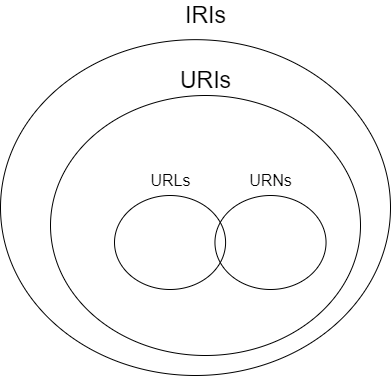
\includegraphics[width=0.5\textwidth]{URI.png}
  \caption{Identifiers}
  \label{fig:uri}
\end{figure}

\begin{lstlisting}[label={lst:uri}, caption={URL and URN examples}]
URL: ftp://ftp.is.co.za/rfc/rfc1808.txt
URL: http://www.ietf.org/rfc/rfc2396.txt
URL: telnet://192.0.2.16:80/
URL: did:ethr:0xb9c5714089478a327f09197987f16f9e5d936e8a
URN: isbn:0-486-27557-4
URN: uuid:6e8bc430-9c3a-11d9-9669-0800200c9a66
\end{lstlisting}


The use of identifiers lets machines to unambiguously refer things in the world. For instance the meaning of the property \lstinline{children} may be obvious for a human-reader depending on the context. If the reader sees the property under a person object, they can infer it means a son or a daughter of that person. However, \lstinline{children} is also used to express hierarchical relationships between things. These semantics need to be stated explicitly for machines to be able to "understand" what these properties stand for and to avoid such ambiguities in machine communication. That's why instead the keys are \acrlong{IRI}s. Also to avoid everyone defining their own \lstinline{child} semantics, vocabularies are defined. One popular vocabulary is \url{schema.org}. To express "a child of a person", the \acrshort{IRI} \url{https://schema.org/children} can be given. In that case a \acrshort{JSON-LD} document looks like in Listing \ref{lst:exampleJSONLD}

\begin{lstlisting}[language=json, label={lst:exampleJSONLD}, caption={A JSON-LD with full \acrshort{IRI}s}]
{
  "@id": "http://doefamily.net/john",
  "http://schema.org/givenName": "John",
  "http://schema.org/familyName": "Doe",
  "http://schema.org/children": {
    "@id": "http://doefamily.net/jane",
    "http://schema.org/givenName": "Jane",
    "http://schema.org/familyName": "Doe"
  }
}
\end{lstlisting}

However this document is difficult to read. Instead of having to write full \acrshort{IRI}s each time, a \lstinline{@context} can be included in the document that will map terms in the included document to \acrshort{IRI}s. Similar to a human communication, this sets the context of the information exchange, thus removing the ambiguity and providing conciseness. A context document for the previous \acrshort{JSON-LD} file might be as follows

\begin{lstlisting}[language=json, label={lst:exampleJSONLD}, caption={A context file}]
{
  "@context": {
    "firstName": "http://schema.org/firstName",
    "lastName": "http://schema.org/lastName",
    "children": "http://schema.org/children"
}
\end{lstlisting}

Assuming the context is located at \lstinline{http://example.com/familyContext}, the previous document becomes more human-readable by embedding the context.

\begin{lstlisting}[language=json, label={lst:exampleJSONLD}, caption={A context added JSON-LD with shortened terms}]
{
    "@context": "http://example.com/familyContext",
    "@id": "http://doefamily.net/john",
    "givenName": "John",
    "familyName": "Doe",
    "children": {
        "@id": "http://doefamily.net/jane",
        "givenName": "Jane",
        "familyName": "Doe"
    }
}
\end{lstlisting}

The examples above are \acrshort{JSON-LD} documents but they are not verifiable credentials. For a document to be a valid verifiable credential they must have the following properties:
\begin{itemize}
    \item A \lstinline{@context} property with the first member \url{https://www.w3.org/2018/credentials/v1}.
    \item A \lstinline{type}\footnote{Alias to \lstinline{@type}, also \lstinline{@id} is aliased to \lstinline{id} in \acrshort{VC}} property that includes the type \lstinline{VerifiableCredential}.
    \item And the following properties: \lstinline{credentialSubject, issuer, issuanceDate, proof}
\end{itemize}

A minimal verifiable credential in \acrshort{JSON-LD} format is shown in Listing \ref{lst:exampleVC}.

\lstinputlisting[language=json, caption={Example verifiable credential \parencite{Sporny.18Kas2019}},label={lst:exampleVC}]{code/exampleVerifiableCredential.json}



%%%%%%
%%%%%%  Public Key Crpyto and Zk proofs
%%%%%% 
\section{Public Key Crypto and JSON-LD}

\subsection{Digital Signatures}

At the heart of today's applications and protocols lies the public key cryptography. The encryption scheme is based on a pair of keys: a public key which can be shared publicly or with the verifying party, and a private key which must be kept absolutely secret except its owner. Hence, it's also called asymmetric cryptography. A user can encrypt a message with their private key, and publish the message and their public key. Anyone anyone can then decrypt the encrypted message with the public key which assures this message was encrypted by the owner of the corresponding private key. Also by encrypting messages with the public key, others can ensure only the owner of the corresponding private key can decrypt the message.

This encryption scheme can also be used to create digital signatures. Apart from the key generation there are two main methods in a digital signature scheme. The \textit{sign} function takes a message and a private key as inputs and generates a signature. The \textit{verify} function takes the message, the digital signature, and the public key as inputs and outputs a boolean value \lstinline{true} if the signature is valid or \lstinline{false} otherwise. Upon receiving a message and a signature, the receiver, if they know the public key of the sender, can check verify it. By verifying the message the receiver can check two things:
\begin{enumerate}
    \item \textbf{Authenticity:} The message is indeed sent by the sender and not someone else
    \item \textbf{Integrity:} The message they receive is indeed the message sender sent and not tampered with
\end{enumerate}

%% Two aspects: signature scheme and key generation (curve)

\subsection{Linked Data Proofs}
\subsection{Zero-Knowledge Proofs}

Zero-knowledge proofs of knowledge are protocols in cryptography where a \textit{prover} can cryptographically prove to a \textit{verifier} the validity of statement without sharing any other information than the fact that the statement is true. The field recently received more attention with the implementation of the privacy-preserving digital currency Zcash \parencite{E.BenSasson.2016}. Even though commonly referred as zero-knowledge proofs, it is useful to distinguish between \textit{proofs} and \textit{proofs of knowledge}. A proof is sufficient evidence for the truth of a proposition such as a proof for the statement that there exists a three coloring for a specific graph. A proof of knowledge is a proof for the knowledge of a piece of information such as a proof to the statement that I know a three coloring for this specific graph \parencite{green_2017}. 

Properties of zero-knowledge proofs are as follows \parencite{Groth.2010}:
\begin{itemize}
  \item \textbf{Completeness:} If the statement is true, the verifier will be convinced by the proof the prover presents that the statement is true
  \item \textbf{Soundness:} If the statement is false, a malicious prover can't convince the verifier that it is true.
  \item \textbf{Zero-Knowledge:} If the statement is true, a malicious verifier does not learn anything else than the fact that the statement is true.
\end{itemize}

The first two properties are also requirements for interactive proofs. The work of \cite{Goldwasser.1985} has first introduced the third property of Zero-Knowledge. A proof in a zero-knowledge proof system is not deterministic but a probabilistic proof. Through many rounds it is possible to decrease the error to practically negligible values. \cite{Goldreich.1991} also show that with the assumption of an unbreakable encryption, it is possible to create a zero-knowledge proof for the graph coloring problem. This is significant since the graph coloring problem is NP-complete and every NP problem can be reduced to an NP-complete problem in polynomial time, meaning every problem in NP has a zero-knowledge proof. 

These initial zero-knowledge proofs are also interactive, that is the prover and the verifier need to exchange information on each round. Each time the a proofs needs to be made, the prover and the verifier need to be online and interact in multiple rounds, which makes the usability of the protocol difficult. Also, since the soundness of the proof relies on the randomness of the challenges of the verifier on each round, a third-party can not be convinced by such a proof. By looking at the protocol transcript and the proof, they can't be assured if this randomness holds. \cite{Blum.1988} have shown that with a common reference string shared by the prover and the verifier, it is possible to create non-interactive zero-knowledge proofs. The common reference string need not be private, which makes non-interactive zero-knowledge proofs more practical than interactive ones.

\section{Related Work}